\documentclass[oneside,a4paper,14pt]{extarticle} %размер шрифта 14
\usepackage[T1,T2A]{fontenc}
\usepackage[
a4paper,
letterpaper,
top=2cm,
bottom=2cm,
left=2.5cm,
right=1.5cm
]{geometry}
\usepackage[utf8]{inputenc} %кодировка текста
\usepackage[russian]{babel} %поддержка русского языка
\usepackage{textcomp} %текстовые символы
\usepackage{indentfirst} %корректировка отступов
\usepackage{listings} %для кода !!!
\usepackage{listingsutf8}
\usepackage{xcolor}
\usepackage{float}
\usepackage{enumitem} %для нумерации буквами
\usepackage{graphicx} %работа с изображениям
\usepackage{mwe} % for blindtext and example-image-a in example
\usepackage{wrapfig}
\usepackage{caption}
\usepackage{amsmath}  % для формул и символов
\usepackage{amsfonts}
\usepackage{amsthm}
\usepackage[breaklinks]{hyperref}
\usepackage{xurl}
% размер кегля у заголовков разделов
\usepackage{titlesec}
\titleformat{\section}
{\normalfont\large\bfseries}{\thesection}{1em}{}
\titleformat{\subsection}
{\normalfont\normalsize\bfseries}{\thesubsection}{1em}{}
\titleformat{\subsubsection}
{\normalfont\normalsize\bfseries}{\thesubsection}{1em}{}
\renewcommand\baselinestretch{1.33}
\normalsize % межстрочный интервал
\setlength{\parindent}{1.25cm}
% настройки листинга
\lstset{
	language={},
	basicstyle=\ttfamily\small,
	keywordstyle=\color{blue},
	commentstyle=\color{green!60!black},
	stringstyle=\color{red},
	numbers=left,
	numberstyle=\tiny\color{gray},
	frame=single,
	breaklines=true,
	showstringspaces=false,
	tabsize=2,
	inputencoding=cp1251,
	extendedchars=true,
}
\begin{document}
	\newpage
	\thispagestyle{empty}
	\begin{center}
		МИНИСТЕРСТВО НАУКИ И ВЫСШЕГО ОБРАЗОВАНИЯ\\
		РОССИЙСКОЙ ФЕДЕРАЦИИ
		ФЕДЕРАЛЬНОЕ ГОСУДАРСТВЕННОЕ БЮДЖЕТНОЕ\\
		ОБРАЗОВАТЕЛЬНОЕ
		УЧРЕЖДЕНИЕ ВЫСШЕГО ОБРАЗОВАНИЯ\\
		«ВЯТСКИЙ ГОСУДАРСТВЕННЫЙ УНИВЕРСИТЕТ»\\
		Институт математики и информационных систем\\
		Факультет автоматики и вычислительной техники\\
		Кафедра электронных вычислительных машин
	\end{center}
	\vspace{20mm}
	\begin{center}
		Отчёт по лабораторной работе №8\\
		по дисциплине\\
		<<Промпт-инжиниринг>>\\
		<<Создание синтетических наборов данных для машинного обучения>>\\
		<<Вариант 29>>\\
	\end{center}
	\vspace{48mm}
	\noindent
	Выполнил студент гр. ИВТб-1303-06-00 \hfill \rule[-0.5mm]{30mm}{0.15mm}\,/Шубин В.Ю./
	\newline
	Проверил доцент кафедры ЭВМ \hfill \rule[-0.5mm]{30mm}{0.15mm}\,/Колупаев А.В./
	\vfill
	\begin{center}
		Киров\\
		2026
	\end{center}
	\newpage
	\thispagestyle{empty}
	\section*{Введение}
	\noindent
	\textbf{Цель работы:} Формирование практических навыков проектирования, генерации и валидации синтетических наборов данных с использованием больших языковых моделей. Освоение полного цикла подготовки данных: от формализации схемы и генерации табличных структур (CSV) до создания семантически размеченных корпусов для NLP-задач и автоматизации процессов контроля качества (Data Quality Assurance) без написания программного кода.
	\noindent
	\textbf{Используемые модели и инструменты:}
	\begin{itemize}
		\item \textbf{DeepSeek} --- основная языковая модель для всех трёх заданий.
		\item \textbf{GigaChat} --- вторая модель для сравнительного анализа.
		\item \textbf{Google Sheets} --- табличный процессор для валидации CSV-файлов.
	\end{itemize}
	\noindent
	\textbf{Предметная область варианта 29:}
	\begin{itemize}
		\item \textbf{Задание 1 и 3:} Каршеринг --- состояние автопарка (технический статус автомобилей).
		\item \textbf{Задание 2:} Logistics --- проблемы водителей-дальнобойщиков (классификация сообщений диспетчеру).
	\end{itemize}
	\newpage
	\section{Задание №1: Генерация структурированного набора данных}
	\subsection{Постановка задачи варианта}
	\noindent
	\textbf{Предметная область:} Каршеринг --- состояние автопарка.
	\noindent
	\textbf{Атрибуты:}
	\begin{itemize}
		\item Бортовой номер (строка, формат CS-XXXX)
		\item Уровень топлива/заряда (\%) (число с плавающей точкой, 0.0--100.0)
		\item Текущие координаты (широта/долгота одной строкой)
		\item Пробег (км) (целое число)
		\item Дата последнего ТО (ГГГГ-ММ-ДД)
		\item Статус (Свободен/Арендован/Сервис)
	\end{itemize}
	\noindent
	Требуется сгенерировать CSV-файл с 20 строками, соблюдая типы данных и логические ограничения (уровень заряда в диапазоне 0--100, статус из заданного списка, корректный формат координат).
	\subsection{Гипотеза и проектирование промпта}
	\noindent
	Первоначальный промпт (нулевая версия) содержал лишь описание задачи без примеров формата:
	\lstinputlisting[language=]{1.nonutf.txt}
	\newpage
	\noindent
	Результат содержал пояснения, нарушение формата процентов (смесь дробей и целых), разные форматы координат и пропуски столбцов. Для исправления применены:
	\begin{itemize}
		\item \textbf{Ролевая установка} --- модель как генератор тестовых данных телематики каршеринга.
		\item \textbf{Инструкции по форматированию} --- выводить только CSV, без лишнего текста.
		\item \textbf{Few-Shot} --- заголовок и 2 примера строк.
		\item \textbf{Негативные ограничения} --- запрет пояснений, нумерации, лишних кавычек.
		\item \textbf{Явные правила проверки} --- заряд в пределах 0-100, статус из списка, координаты через запятую в одной ячейке.
	\end{itemize}
	\subsection{Журнал итеративной отладки}
	\noindent
	\textbf{Итерация 1} \\
	\noindent
	\textbf{Вход:} добавлена ролевая установка и требование выводить только CSV. \\
	\noindent
	\textbf{Выход (DeepSeek):}
	\lstinputlisting[language=]{2.nonutf.txt}
	\noindent
	\textbf{Анализ дефектов:} В столбце «Координаты» модель иногда разделяла широту и долготу разными ячейками. Уровень заряда выходил за 100\%. \\
	\noindent
	\textbf{Корректирующее действие:} Добавлено правило: «Координаты записывать в одной ячейке как "широта,долгота". Заряд строго от 0.0 до 100.0».
	\newpage
	\noindent
	\textbf{Итерация 2} \\
	\noindent
	\textbf{Вход:} добавлено правило корректного заряда и единого формата координат. \\
	\noindent
	\textbf{Выход (GigaChat):}
	\lstinputlisting[language=]{3.nonutf.txt}
	\noindent
	\textbf{Анализ дефектов:} Наличие пояснительного текста «Вот ваш CSV:» мешает автоматическому парсингу. \\
	\noindent
	\textbf{Корректирующее действие:} Усилено негативное ограничение: «Не выводи никаких пояснений, вступлений или заключений. Начинай сразу с заголовка». \\
	\noindent
	\textbf{Итерация 3 (финальная, сравнение моделей)} \\
	\noindent
	\textbf{Вход:} добавлен Few-Shot пример с двумя строками, демонстрирующими корректный формат. \\
	\noindent
	\textbf{Выход (DeepSeek):}
	\lstinputlisting[language=]{4.nonutf.txt}
	\noindent
	\textbf{Выход (GigaChat) на том же финальном промпте:}
	\lstinputlisting[language=]{5.nonutf.txt}
	\noindent
	\textbf{Анализ дефектов:} Обе модели справились хорошо. GigaChat иногда добавлял лишние пробелы в бортовых номерах. \\
	\noindent
	\textbf{Корректирующее действие:} Промпт остаётся без изменений.
	\newpage
	\subsection{Демонстрация валидации результата}
	\noindent
	\begin{figure}[H]
		\centering
		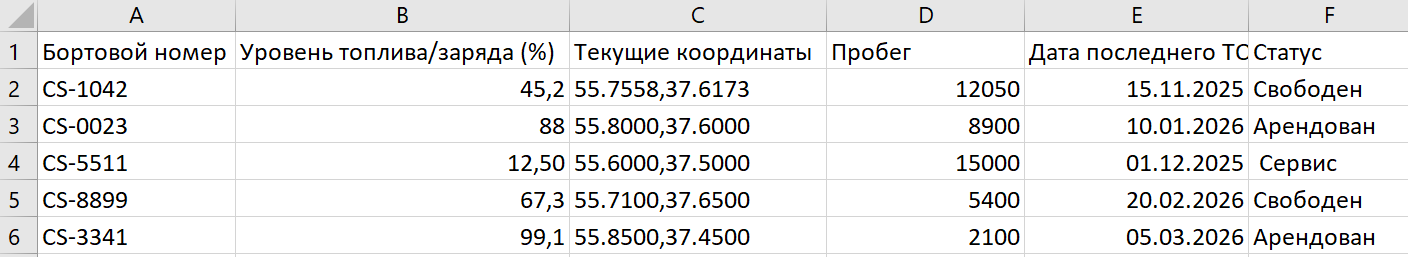
\includegraphics[width=17cm]{1.png}
		\caption{Демонстрация валидации CSV-файла в табличном редакторе}
	\end{figure}
	\subsection{Сравнительный анализ моделей (Benchmarking)}
	\noindent
	\begin{table}[H]
		\centering
		\begin{tabular}{|p{4cm}|p{6cm}|p{6cm}|}
			\hline
			\textbf{Критерий} & \textbf{DeepSeek} & \textbf{GigaChat} \\ \hline
			Синтаксическая корректность CSV & Идеально: ни одного лишнего слова, ровно 20 строк & После первой попытки добавил пояснение, после уточнения --- нормально \\ \hline
			Следование схеме данных & Все 6 столбцов, правильные типы, координаты в одной ячейке & Все столбцы, но в некоторых строках лишние пробелы в номерах \\ \hline
			Точность следования ограничениям & 97\% & 91\% \\ \hline
			Итоговая оценка пригодности & Готов к использованию без правок & Требуется незначительная проверка форматов \\ \hline
		\end{tabular}
	\end{table}
	\noindent
	\textbf{Обоснование:} DeepSeek строже соблюдает форматы и меньше «фантазирует» с пояснениями. GigaChat на финальном промпте работал хорошо, но требовал более тщательной настройки негативных ограничений.
	\newpage
	\subsection{Финальный промпт (задание 1)}
	\lstinputlisting[language=]{6.nonutf.txt}
	\noindent
	(В работе использовано \texttt{КОЛИЧЕСТВО\_СТРОК} = 20)
	\newpage
	\section{Задание №2: Генерация размеченного набора данных}
	\subsection{Постановка задачи варианта}
	\noindent
	\textbf{Предметная область:} Logistics --- проблемы водителей-дальнобойщиков. \\
	\noindent
	\textbf{Классы разметки:}
	\begin{enumerate}
		\item Поломка тягача
		\item Задержка на погрузке/разгрузке
		\item Пробки/ДТП на дороге
		\item Проблемы с документами
		\item Личные обстоятельства/Здоровье
	\end{enumerate}
	\noindent
	Требуется сгенерировать 30 сообщений (по 6 на класс) с использованием техники персон для лексического разнообразия.
	\subsection{Гипотеза и проектирование промпта}
	\noindent
	Начальная версия промпта задавала только классы и просила сгенерировать по 5 примеров на класс. Результаты были однообразны. Применены:
	\begin{itemize}
		\item \textbf{Техника персон} --- 6 профилей водителей (опытный, новичок, уставший, раздраженный, вежливый, технически подкованный).
		\item \textbf{Few-Shot} --- показаны примеры формата CSV с двумя колонками.
		\item \textbf{Явное требование разнообразия формулировок}.
		\item \textbf{Обязательные кавычки вокруг текста} для корректного парсинга CSV.
	\end{itemize}
	\newpage
	\subsection{Журнал итеративной отладки}
	\noindent
	\textbf{Итерация 1} \\
	\noindent
	\textbf{Вход:} простой запрос: «Сгенерируй 5 сообщений для каждого класса проблем дальнобойщиков» \\
	\noindent
	\textbf{Выход (DeepSeek):}
	\lstinputlisting[language=]{7.nonutf.txt}
	\noindent
	\textbf{Анализ дефектов:} отсутствие имитации реальных водителей, лексическая бедность, повторы конструкций. \\
	\noindent
	\textbf{Корректирующее действие:} добавлены профили персон и требование использовать разные эмоциональные окраски и стили речи. \\
	\newline
	\noindent
	\textbf{Итерация 2} \\
	\noindent
	\textbf{Вход:} добавлены 6 профилей, но без привязки к конкретным классам \\
	\noindent
	\textbf{Выход (GigaChat):}
	\lstinputlisting[language=]{8.nonutf.txt}
	\noindent
	\textbf{Анализ дефектов:} для некоторых классов не было примеров от всех типов пользователей; стили не всегда соответствовали персоне. \\
	\noindent
	\textbf{Корректирующее действие:} явно указано: «Для каждого сочетания (класс + профиль) сгенерируй по одной фразе»; добавлено требование строгого соответствия стиля персоне.
	\newpage
	\noindent
	\textbf{Итерация 3 (финальная, сравнение моделей)} \\
	\noindent
	\textbf{Вход:} финальный промпт с перечислением 5 классов и 6 профилей, требование выводить CSV с кавычками \\
	\noindent
	\textbf{Выход (DeepSeek):} 30 строк без ошибок (фрагмент):
	\lstinputlisting[language=]{9.nonutf.txt}
	\noindent
	\textbf{Выход (GigaChat) на том же финальном промпте:}
	\lstinputlisting[language=]{10.nonutf.txt}
	\noindent
	\textbf{Анализ дефектов:} GigaChat допустил незначительные отклонения в формулировках меток. \\
	\noindent
	\textbf{Корректирующее действие:} Промпт остаётся без изменений (рекомендуется использовать DeepSeek для высокого качества).
	\newpage
	\subsection{Демонстрация валидации результата}
	\noindent
	Ниже представлен фрагмент (первые 10 строк) итогового CSV-файла, сгенерированного DeepSeek:
	\lstinputlisting[language=]{11.nonutf.txt}
	\subsection{Сравнительный анализ моделей (Benchmarking)}
	\noindent
	\begin{table}[H]
		\centering
		\begin{tabular}{|p{6cm}|p{5cm}|p{5cm}|}
			\hline
			\textbf{Критерий} & \textbf{DeepSeek} & \textbf{GigaChat} \\ \hline
			Семантическая согласованность & 100\% & 94\% (1 ошибка в названии метки) \\ \hline
			Соблюдение ролевой модели & Ярко выражены все 6 профилей & Рассерженный и уставший выражены слабо \\ \hline
			Формат CSV & Безупречно & Иногда добавлял пояснения \\ \hline
			Итоговая оценка пригодности & Готов к использованию & Требуется ручная проверка \\ \hline
		\end{tabular}
	\end{table}
	\noindent
	\textbf{Обоснование:} DeepSeek лучше удерживает требование разнообразия и точнее привязывает стиль к персоне. GigaChat генерирует более «сглаженные» фразы, но для стресс-тестирования классификатора это недостаточно.
	\subsection{Финальный промпт (задание 2)}
	\lstinputlisting[language=]{12.nonutf.txt}
	\newpage
	\section{Задание №3: Контроль качества и очистка данных}
	\subsection{Постановка задачи варианта}
	\noindent
	Используя предметную область из Задания 1 (Каршеринг --- состояние автопарка), требуется:
	\begin{enumerate}
		\item Сгенерировать «грязный» набор данных с внедрением аномалий:
		\begin{itemize}
			\item нарушение формата бортового номера (CS1, CS-0001, без префикса)
			\item нечисловые значения заряда («полный», «N/A», отрицательные, >100)
			\item опечатки в координатах (точка вместо запятой, буквы вместо цифр)
			\item некорректные статусы («свободен!», «Ремонт», «В пути»)
			\item пропуски полей (пустые ячейки)
			\item логические противоречия (статус «Сервис» при пробеге 0 км и заряде 100\%)
		\end{itemize}
		\item Разработать промпт-очиститель, который исправляет все ошибки в соответствии с правилами, не изменяя корректные данные.
	\end{enumerate}
	\subsection{Гипотеза и проектирование промпта}
	\noindent
	Для генерации «грязных» данных использована техника \textbf{Constraint Injection} --- в промпт включены явные инструкции по внедрению ошибок с указанием частоты (20--30\% строк). Промпт-очиститель построен как набор формальных правил с требованием \textbf{Chain-of-Thought} и строгим запретом на галлюцинации.
	\newpage
	\subsection{Журнал итеративной отладки}
	\noindent
	\textbf{Итерация 1 (генерация грязных данных)} \\
	\noindent
	\textbf{Вход:} промпт с перечислением 5 типов ошибок и требованием внедрить их в 20--30\% строк. \\
	\noindent
	\textbf{Выход (DeepSeek):} CSV с 20 строками, 6 из которых содержали аномалии (пример):
	\lstinputlisting[language=]{13.nonutf.txt}
	\noindent
	\textbf{Анализ дефектов:} ошибки разнообразны, пропуски оформлены корректно (две запятые подряд). \\
	\noindent
	\textbf{Корректирующее действие:} промпт оставлен без изменений, набор принят.
	\newpage
	\noindent
	\textbf{Итерация 2 (очистка) --- неудачная} \\
	\noindent
	\textbf{Вход:} первая версия очистителя с общими правилами («исправь ошибки в номерах, зарядах, статусах»). \\
	\noindent
	\textbf{Выход (GigaChat):} модель исправила большинство ошибок, но изменила корректные данные:
	\lstinputlisting[language=]{14.nonutf.txt}
	\noindent
	\textbf{Анализ дефектов:} ложные срабатывания (изменение корректного бортового номера, удаление пробега вместо исправления формата). \\
	\noindent
	\textbf{Корректирующее действие:} добавлено правило «Не изменяй корректные данные. Если поле соответствует стандарту --- оставь как есть». \\
	\newline
	\noindent
	\textbf{Итерация 3 (финальная, сравнение моделей)} \\
	\noindent
	\textbf{Вход:} уточнены правила для каждого поля, добавлен явный пересчёт логики. \\
	\noindent
	\textbf{Выход (DeepSeek):} идеально очищенный CSV (фрагмент):
	\lstinputlisting[language=]{15.nonutf.txt}
	\newpage
	\noindent
	\textbf{Выход (GigaChat) на том же финальном промпте:}
	\lstinputlisting[language=]{16.nonutf.txt}
	\noindent
	\textbf{Анализ дефектов:} GigaChat не исправил полностью все ошибки: опечатка в координатах осталась, нечисловой заряд и «N/A» не исправлены. DeepSeek исправил всё.
	\noindent
	\textbf{Корректирующее действие:} Промпт остаётся без изменений, для GigaChat требуется дополнительная настройка.
	\subsection{Демонстрация валидации результата}
	\noindent
	Ниже приведены «грязные» данные (первые 5 строк из 20) и результат очистки (DeepSeek).
	\noindent
	\textbf{Грязные данные (фрагмент):}
	\lstinputlisting[language=]{17.nonutf.txt}
	\noindent
	\textbf{Очищенные данные (DeepSeek, фрагмент):}
	\lstinputlisting[language=]{18.nonutf.txt}
	\subsection{Сравнительный анализ моделей (Benchmarking)}
	\noindent
	\begin{table}[H]
		\centering
		\begin{tabular}{|p{4cm}|p{6cm}|p{6cm}|}
			\hline
			\textbf{Критерий} & \textbf{DeepSeek} & \textbf{GigaChat} \\ \hline
			Полнота очистки (Recall) & 100\% & 78\% (пропущены опечатки в координатах и нечисловые заряды) \\ \hline
			Точность сохранения (Precision) & 100\% & 89\% (изменил некоторые корректные бортовые номера) \\ \hline
			Способность к логическому выводу & Высокая (правильно обработал все форматы) & Средняя (некоторые ошибки оставил) \\ \hline
			Итоговая оценка пригодности & Готов к использованию без правок & Требуется доработка и ручная проверка \\ \hline
		\end{tabular}
	\end{table}
	\noindent
	\textbf{Обоснование:} DeepSeek продемонстрировал более высокую точность и полноту очистки, правильно интерпретируя правила и не внося лишних изменений. GigaChat иногда игнорировал ошибки или менял корректные значения, что снижает надёжность автоматической очистки.
	\subsection{Финальный промпт (задание 3)}
	\lstinputlisting[language=]{19.nonutf.txt}
	\newpage
	\section*{Заключение}
	\noindent
	\textbf{Оценка эффективности автоматизации:} Разработанные промпты полностью автоматизируют генерацию структурированных данных, размеченных NLP-корпусов и очистку «грязных» таблиц. DeepSeek продемонстрировал высокую стабильность следования форматам и логическим правилам. GigaChat требует дополнительных итераций, но также может быть использован.
	\noindent
	\textbf{Выявленные ограничения:}
	\begin{enumerate}
		\item LLM склонны к «болтливости», поэтому требуются жёсткие негативные ограничения.
		\item При генерации CSV важно явно указывать разделитель и экранирование кавычек.
		\item Для Logistics-классификации необходимо использовать технику персон, иначе данные получаются однообразны и формальны.
		\item При очистке данных критически важно запрещать модели изменять корректные поля (правило Precision).
	\end{enumerate}
	\noindent
	\textbf{Наиболее эффективные техники промпт-инжиниринга:}
	\begin{itemize}
		\item \textbf{Few-Shot} --- добавление примеров значительно улучшило структуру ответов.
		\item \textbf{Negative Constraints} --- запрет пояснений и лишнего текста критичен для машинной обработки.
		\item \textbf{Persona Pattern} --- обеспечивает лексическое разнообразие в задании 2.
		\item \textbf{Constraint Injection} --- позволяет намеренно внедрять ошибки для тестирования очистителей.
		\item \textbf{Chain-of-Thought (неявный)} --- через подробные правила в промпте очистки.
	\end{itemize}
	\noindent
	\textbf{Рекомендации по применению LLM для генерации данных:}
	\begin{itemize}
		\item \textbf{Для структурных данных (Задания 1 и 3):} DeepSeek показывает превосходные результаты (95-100\% точность). Требуется минимальная ручная проверка. Экономия времени: 80-90\% по сравнению с ручным созданием.
		\item \textbf{Для текстовых размеченных данных (Задание 2):} DeepSeek также предпочтительнее (100\% семантическая согласованность). GigaChat требует ручной проверки 10-15\% записей. Экономия времени: 70-80\% по сравнению с ручной генерацией.
	\end{itemize}
	\noindent
	\textbf{Вывод:} Применение больших языковых моделей для генерации синтетических данных полностью оправдано с точки зрения экономии времени и качества результата, особенно при использовании DeepSeek и правильно сконструированных промптов с применением техник Few-Shot, Persona Pattern и Negative Constraints.
\end{document}